\documentclass{article}
\usepackage[margin=0.6in]{geometry}
\usepackage{amsmath}
\usepackage{amssymb}
\usepackage{bookmark}
\usepackage{graphicx}
\usepackage{float}

\newcommand{\vct}[1]{\mathbf{#1}}
\newcommand{\argmax}{\mathop{\mathrm{argmax}}}
\newcommand{\argmin}{\mathop{\mathrm{argmin}}}

\title{Solutions to the Assignment - 5 : CS5560 - \\
Probabilistic Models in Machine Learning}
\author{Vishwak Srinivasan\\
\texttt{CS15BTECH11043}}
\date{}

\begin{document}
\maketitle

\section*{Exercises from ML: A Probabilistic Perspective}
\subsection*{Exercise 4.19}
\begin{flushleft}
\end{flushleft}

\subsection*{Exercise 4.21}
\subsubsection*{Part a}
\begin{flushleft}
If \(p(x | \mu_{1}, \sigma_{1}) \geq p(x | \mu_{2}, \sigma_{2})\), then \(-2\log p(x | \mu_{1}, \sigma_{1}) \leq -2\log p(x | \mu_{2}, \sigma_{2})\). This means that:
\begin{equation}
\label{r1-eqn}
\frac{(x - \mu_{1})^{2}}{\sigma_{1}^{2}} + \log \sigma_{1}^{2} \leq \frac{(x - \mu_{2})^{2}}{\sigma_{2}^{2}} + \log \sigma_{2}^{2} \Rightarrow x^2 - \frac{(x - 1)^{2}}{10^{6}} - \log (10^{6}) \leq 0 \Rightarrow x^{2}\left(1 - \frac{1}{10^{6}}\right) + x\frac{2}{10^{6}} - \left(\frac{1}{10^{6}} + \log 10^{6}\right) \leq 0
\end{equation}

A graphical sketch is shown below:
\(\newline\)
\begin{minipage}{0.475\linewidth}
\begin{figure}[H]
\centering
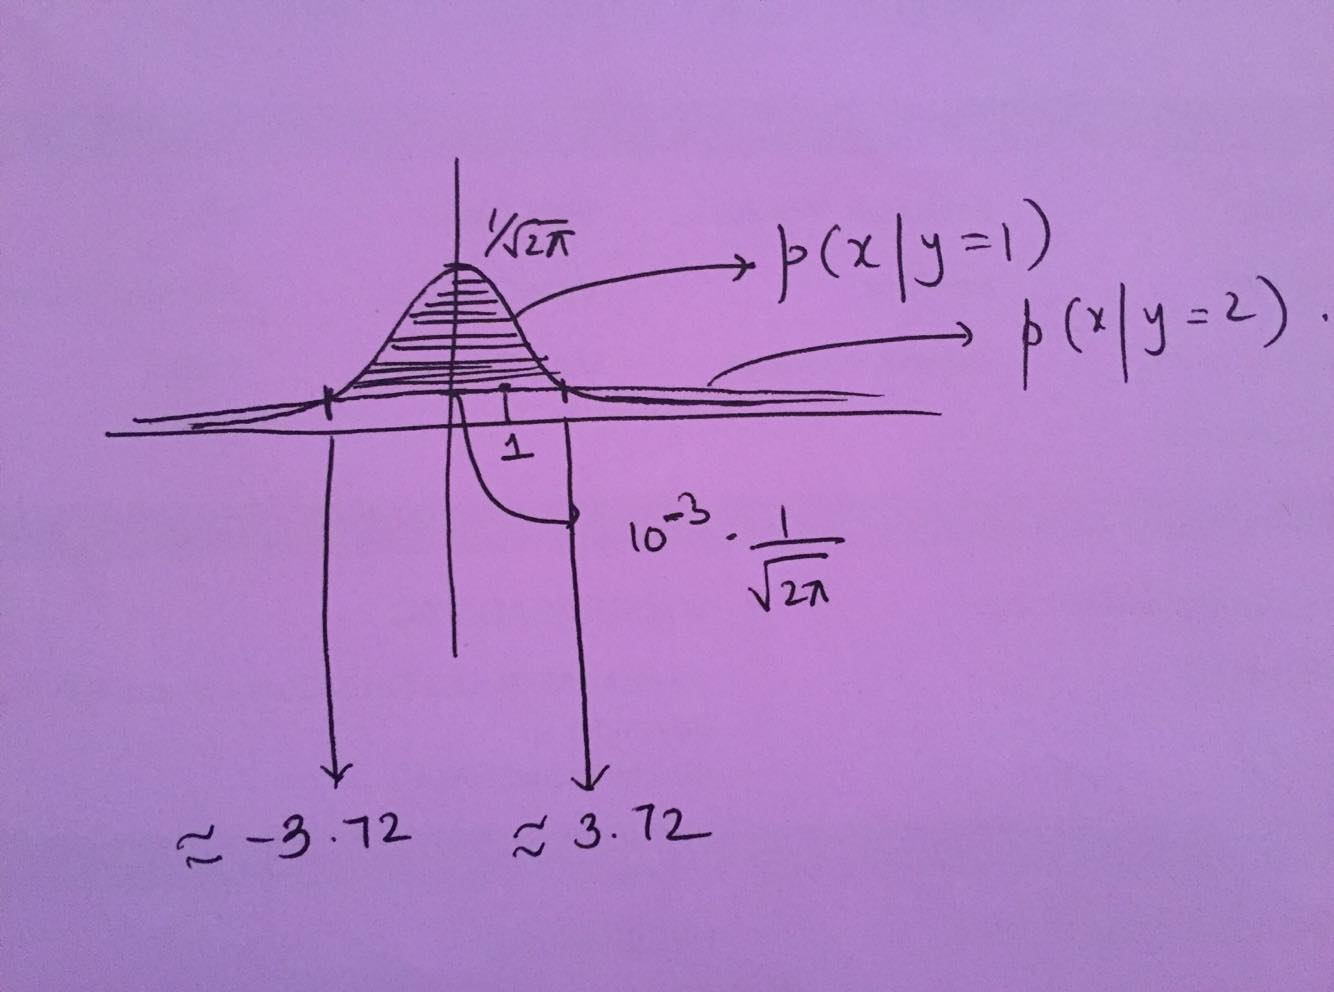
\includegraphics[width=0.6\textwidth]{./images/4_21_a_sketch.jpg}
\end{figure}
\end{minipage}
\hfill
\begin{minipage}{0.475\linewidth}
The domain of the shaded region corresponds to the set \(R_{1}\). The end-points of this domain can be found by solving the equality case in \ref{r1-eqn}. Denote \(C_{1} = 1 - \frac{1}{10^{6}}\), \(C_{2} = \frac{2}{10^{6}}\) and \(C_{3} = -\left(\frac{1}{10^{6}} + \log 10^{6}\right)\).
\begin{multline}
C_{1}x^2 + C_{2}x + C_{3} = 0 \Rightarrow x = \frac{-C_2 \pm \sqrt{C_{2}^{2} - 4C_{1}C_{3}}}{2C_{1}}\\= \frac{-1 \pm 10^{3}\sqrt{10^{6}\log 10^{6} + 1 - \log 10^{6}}}{(10^{6} - 1)}\\\Rightarrow x \approx \pm 3.7169
\end{multline}
\end{minipage}
\end{flushleft}

\subsubsection*{Part b}
\begin{flushleft}
Note that if \(\sigma_{1}^{2} = \sigma_{2}^{2}\), then the first equality in \ref{r1-eqn} would become:
\begin{equation}
(x - \mu_{1})^{2} \leq (x - \mu_{2})^{2} \Rightarrow 2(\mu_{2} - \mu_{1})x \leq \mu_{2}^{2} - \mu_{1}^{2} \Rightarrow x \leq \frac{\mu_{2} + \mu_{1}}{2} = \frac{1}{2}
\end{equation}

\begin{minipage}{0.475\linewidth}
\begin{figure}[H]
\centering
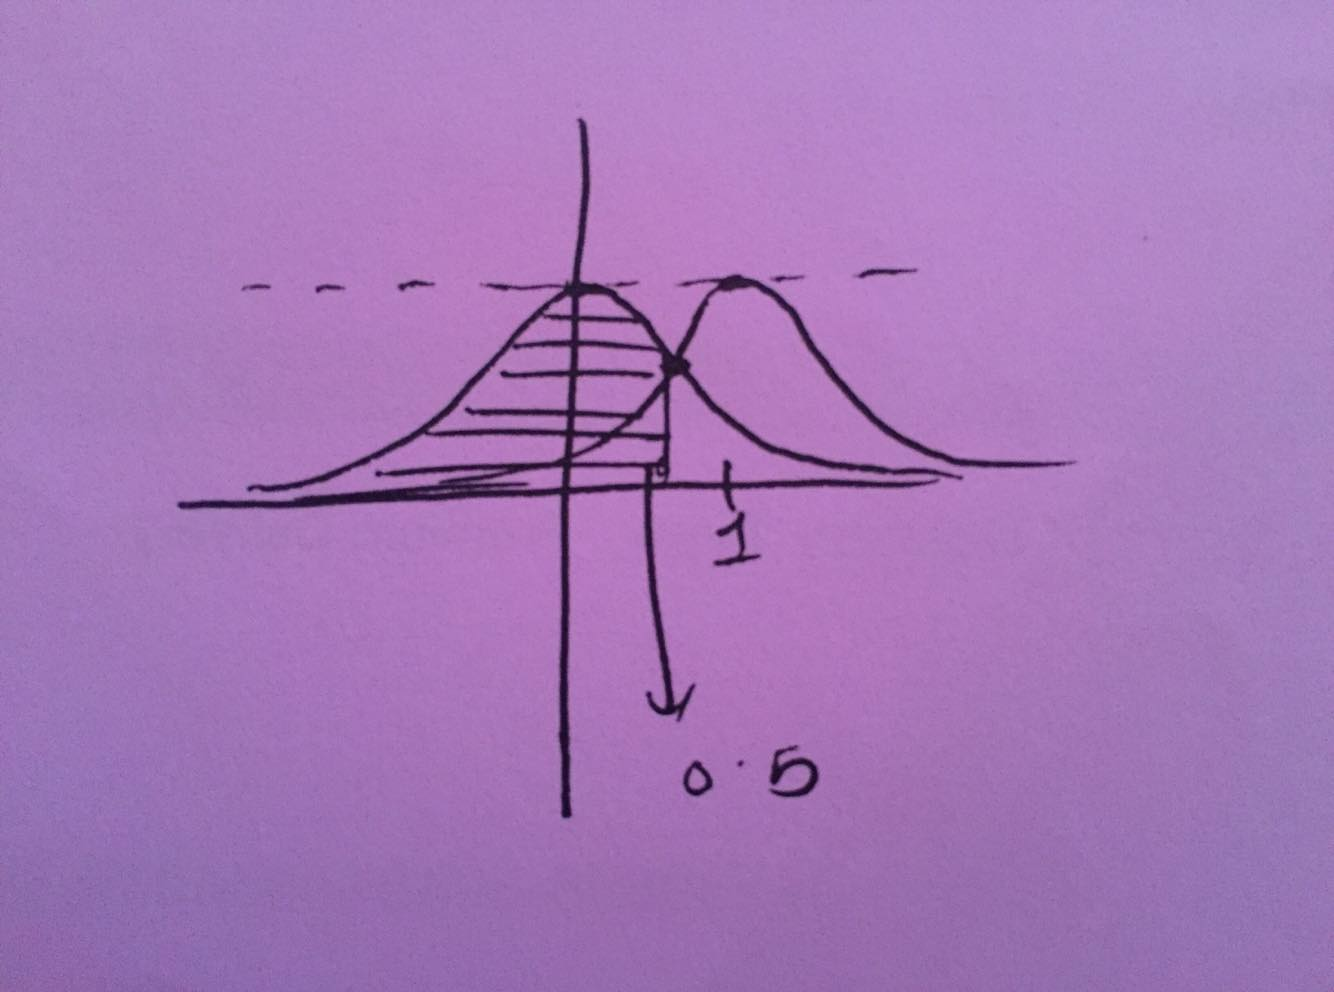
\includegraphics[width=0.6\textwidth]{./images/4_21_b_sketch.jpg}
\end{figure}
\end{minipage}
\hfill
\begin{minipage}{0.475\linewidth}
\(R_{1}\) is the left partition of the real line from \(\frac{1}{2}\).
\end{minipage}
\end{flushleft}

\subsection*{Exercise 4.22}
\begin{flushleft}
Recall that the predictor is given by \(\hat{g}(\vct{x}) = \argmax_{y \in \mathcal{Y}} p(Y | \vct{x} = y)\). Now from the facts in the question:
\begin{equation}
p(y | \vct{x}) \propto p(\vct{x} | y) p(y) \propto p(\vct{x} | y)
\end{equation}

The last proportionality excludes \(p(y)\) due to the fact that the \(P(Y = 1) = P(Y = 2) = P(Y = 3) = \frac{1}{3}\). Now the prediction equation can be re-written as:
\begin{equation}
\hat{g}(\vct{x}) = \argmax_{y \in \{1, 2, 3\}} p(\vct{x} | Y = y) = \argmax_{y \in \{1, 2, 3\}} \log p(\vct{x} | Y = y) = \argmin_{y \in \{1, 2, 3\}} -2\log p(\vct{x} | Y = y) - \log 2\pi
\end{equation}

Some equations to consider:
\begin{gather}
-2\log p(\vct{x} | Y = i) - \log 2\pi= (\vct{x} -\vct{\mu}_{1})^{T}\Sigma^{-1}_{1}(\vct{x} -\vct{\mu}_{1}) + 2\log |\Sigma_{i}|
\end{gather}

\begin{center}
\begin{tabular}{|c|c|c|}
\hline
\(i\) & \(\Sigma_{i}^{-1}\) & \(|\Sigma_{i}|\) \\
\hline
\(1\) & \(\begin{bmatrix} \frac{1}{0.7} & 0 \\ 0 & \frac{1}{0.7} \end{bmatrix}\) & \(0.49\) \\
\hline
\(2\) & \(\begin{bmatrix} \frac{4}{3} & -\frac{1}{3} \\ -\frac{1}{3} & \frac{4}{3} \end{bmatrix}\) & \(0.6\) \\
\hline
\(3\) & \(\begin{bmatrix} \frac{4}{3} & -\frac{1}{3} \\ -\frac{1}{3} & \frac{4}{3} \end{bmatrix}\) & \(0.6\) \\
\hline
\end{tabular}
\end{center}

\subsubsection*{Part a}
\begin{equation}
\hat{g}([-0.5, 0.5]) = \argmin_{y \in \{1, 2, 3\}} \{1.69, 4.03, 2.03\} = 1
\end{equation}

\subsubsection*{Part b}
\begin{equation}
\hat{g}([0.5, 0.5]) = \argmin_{y \in \{1, 2, 3\}} \{1.69, 1.7, 5.03\} = 1
\end{equation}
\end{flushleft}
\end{document}
